\chapter{Parareal Method}
\label{sec:pr}

The parareal method is a parallel-in-time integration scheme to solve \acp{ODE}.
It goes back to \citeauthor{Lions2001}~\cite{Lions2001},
though the most common form also used in this thesis first appeared in \citeauthor{Baffico2002}~\cite{Baffico2002}.
This chapter first describes the general properties of the parareal method,
and derives it as a Newton method following \citeauthor{Gander2007}~\cite{Gander2007}.
Lastly, \autoref{sec:pr:DRE} adapts the method for \acp{LRSIF}.

\section{Overview}
\label{sec:pr:properties}

Consider the autonomous \ac{IVP}
\begin{equation}
  \label{eq:IVP}
  \left\{
  \begin{aligned}
    \dot u &= f(u) \\
    u(t_0) &= u_0
  \end{aligned}
  \right.
\end{equation}
over the time span $[t_0, t_f]$.
In practical applications,
one is typically interested in a high temporal resolution trajectory of $u$.
Let $F(t, t_0, u_0) \approx u(t)$ be such a fine/high-precision solver for the \ac{IVP} above.
However, applying $F$ to the whole time span may be too slow.
The goal therefore is to apply $F$ on several time slices $[t_{n-1}, t_n]$ in parallel,
$1 \leq n \leq N$,
with the help of a faster but lower-precision solver $G(t, t_0, u_0) \approx u(t)$.
Therefore, fix a coarse discretization $t_0 < t_1 < \ldots < t_N = t_f$.
Then the parareal method to compute $U_n \approx u(t_n)$ reads
\begin{equation}
  \label{eq:pr:method}
  \left\{
  \begin{aligned}
    U^0_{n+1} &:= G(U^0_n) \\
    U^{k+1}_{n+1} &:= G(U^{k+1}_n) + F(U^k_n) - G(U^k_n)
  \end{aligned}
  \right.
\end{equation}
where $U^*_0 := u_0$ and $G(U_n) := G(t_{n+1}, t_n, U_n)$,
$F(U_n) := F(t_{n+1}, t_n, U_n)$
integrate from~$t_n$ to~$t_{n+1}$.
The general data dependencies between the parareal iterates~$U_n^k$
are shown in \autoref{fig:pr:DAG}.
Observe that in any topological order of that graph,
the coarse solutions $G(U_n^k)$ for any fixed~$k$ need to be computed sequentially over $n$.

Notice how in general each coarse solution $G(\optional{})$ is needed twice.
Therefore, a reasonable scheduling pattern of the directed acyclic graph of \autoref{fig:pr:DAG}
that exploits good data locality is a pipeline of stages $n$ which compute
\begin{equation}
\label{eq:pr:stage}
  \begin{tikzpicture}[
    baseline=(Un1k1.base),
    text height=1.5ex,
    text depth=0.25ex,
  ]
    \graph[grow right sep=0] {
      ""/"\ldots,"
      -!- Gnk1/"$G(U_{n-1}^{k})$\rlap{,}"
      -!- Un1k1/"$U_{n}^{k}$\rlap{,}"
      -!- Fnk/"$F(U_{n-1}^{k})$,"
      -!- ""/"\ldots,"
    };
    \draw[<-] (Gnk1) -- +(70:-1cm);
    \draw[->] (Un1k1) -- +(70:1cm);
  \end{tikzpicture}
\end{equation}
where the arrows denote data dependencies or transmissions from and to the adjacent stages.
Dependencies within a stage are not shown.
Note how this pattern correspond to the rows of \autoref{fig:pr:DAG}.
Each stage~$n$ holds~$G(U_{n-1}^{k-1})$ and~$F(U_{n-1}^{k-1})$ in memory,
receives~$U_{n-1}^k$ from its predecessor,
and sends~$U_n^k$ to its successor.
However, there is no need that all stages $n$ compute the same number of refinements $k$,
due to the following proposition.

\begin{figure}[t]
  \centering
  \begin{tikzpicture}[
  text height=1.5ex,
  text depth=0.25ex,
]
  \graph[
    math nodes,
    chain shift={(70:1.2cm)},
    %chain shift={(90:1cm)},
    group shift={(2cm,0)},
    diag/.style={out=30,in=180},
    %diag/.style={bend left=15},
  ]{
    Unk/"U_{n-1}^{k-1}"
    -> Gnk/"G(U_{n-1}^{k-1})" -> Un1k/"U_{n}^{k-1}"
    -> Gn1k/"G(U_{n}^{k-1})" -> Un2k/"U_{n+1}^{k-1}",
    "" -!- Fnk/"F(U_{n-1}^{k-1})" -!- "" -!- Fn1k/"F(U_{n}^{k-1})",
    Unk1/"U_{n-1}^{k}"
    -> Gnk1/"G(U_{n-1}^{k})" -> Un1k1/"U_{n}^{k}"
    -> Gn1k1/"G(U_{n}^{k})" -> Un2k1/"U_{n+1}^{k}",
    "" -!- Fnk1/"F(U_{n-1}^{k})" -!- "" -!- Fn1k1/"F(U_{n}^{k})",
    Unk2/"U_{n-1}^{k+1}"
    -> Gnk2/"G(U_{n-1}^{k+1})" -> Un1k2/"U_{n}^{k+1}"
    -> Gn1k2/"G(U_{n}^{k+1})" -> Un2k2/"U_{n+1}^{k+1}";

    Unk -> Fnk -> Un1k1 -> Fn1k1 -> Un2k2;
    Un1k -> Fn1k -> Un2k1;
    Unk1 -> Fnk1 -> Un1k2;
    Gnk -> [diag] Un1k1;
    Gnk1 -> [diag] Un1k2;
    Gn1k -> [diag] Un2k1;
    Gn1k1 -> [diag] Un2k2;
  };
  \foreach \n in {Unk,Unk1,Unk2} {
    \draw (\n)++(70:-6mm) node[rotate=70] {$\cdots$};
  }
  \foreach \n in {Un2k,Un2k1,Un2k2} {
    \draw (\n)++(70:6mm) node[rotate=70] {$\cdots$};
  }
  \foreach \n in {Unk2,Un1k2,Un2k2} {
    \node [right=4mm] at (\n) {$\cdots$};
  }
  \foreach \n in {Unk,Un1k,Un2k} {
    \node [left=4mm] at (\n) {$\cdots$};
  }
\end{tikzpicture}

  \caption{Dependencies between parareal values $U^{k}_{n}$}
  \label{fig:pr:DAG}
\end{figure}

\begin{proposition}[Diagonal Convergence]
\label{thm:pr:conv}
  Stage $n$ of the parareal method converges after at most $k=n$ iterations:
  \begin{equation*}
    U^k_n = U^n_n = F(U^{n-1}_{n-1})
    \quad
    \forall k \geq n
  \end{equation*}
\end{proposition}
\begin{proof}
  Due to $U^k_0 = u_0$ for all $k$,
  it follows by induction $\forall k \geq n$:
  \begin{equation*}
    \begin{array}{r@{}l@{}l@{}l}
      U^{k+1}_{n+1}
      :={} & F(U^k_n) &{}+ G(U^{k+1}_n) &{}- G(U^k_n) \\
      ={}  & F(U^n_n) &{}+ G(U^n_n)     &{}- G(U^n_n)
      = F(U^n_n)
    \end{array}
  \end{equation*}
\end{proof}

The early iterates $U_n^k$ for $k=n$ thus have fewer dependencies between them,
\cf \autoref{fig:pr:DAG:early}.
Furthermore, the same reasoning as in the proof of \autoref{thm:pr:conv} can
be applied if stage $n$ converges after refinement $k < n$,
\ie $U^{k+1}_n \approx U^k_n$.
In that case, stage $n+1$ converges the refinement thereafter,
\begin{equation}
  \begin{array}{r@{}l@{}l@{}l}
    U^{k+1}_{n+1}
    :={}      & F(U^k_n) &{}+ G(U^{k+1}_n) &{}- G(U^k_n) \\
    \approx{} & F(U^k_n) &{}+ G(U^k_n)     &{}- G(U^k_n)
    = F(U^k_n)
    .
  \end{array}
\end{equation}
Therefore,
assuming $G$ is well conditioned,
there is no need to compute $G(U^{k+1}_n)$.

\begin{figure}[t]
  \centering
  \begin{tikzpicture}[
  text height=1.5ex,
  text depth=0.25ex,
  double equal sign distance,
  ghost/.style={gray},
  eq/.style={double, shorten >=2ex, shorten <=2ex},
]
  \graph[
    math nodes,
    chain shift={(70:1.2cm)},
    group shift={(2cm,0)},
    diag/.style={out=30,in=180},
  ]{
    Unk/"U_0^0"
    -> Gnk/"G(U_0^0)" -> Un1k/"U_1^0"
    -> Gn1k/"G(U_1^0)" -> Un2k/"U_2^0",
    Unk1/"U_0^1" [ghost]
    -!- Fnk/"F(U_0^0)" -!- "" -!- Fn1k/"F(U_1^0)",
    "" -!- "" -!- Un1k1/"U_1^1"
    -> Gn1k1/"G(U_1^1)" -> Un2k1/"U_2^1",
    "" -!- "" -!- Un1k2/"U_1^2" [ghost]
    -!- Fn1k1/"F(U_1^1)",
    "" -!- "" -!- "" -!- "" -!- Un2k2/"U_2^2";

    Unk -> Fnk -> Un1k1 -> Fn1k1 -> Un2k2;
    Un1k -> Fn1k -> Un2k1;
    Gn1k -> [diag] Un2k1;

    Unk -- [ghost,eq] Unk1;
    Un1k1 -- [ghost,eq] Un1k2;
  };
  \draw[ghost] (Un2k2) ++ (2cm,0) node (Un2k3) {$U_2^3$};
  \draw[ghost,eq] (Un2k2) -- (Un2k3);

  \foreach \n in {Un2k,Un2k1,Un2k2} {
    \draw (\n)++(70:6mm) node[rotate=70] {$\cdots$};
  }
  \foreach \n in {Unk1,Un1k2,Un2k3} {
    \node[ghost,right=3mm] at (\n) {$\cdots$};
  }
\end{tikzpicture}

  \caption{Dependencies between parareal values $U^0_0, \ldots, U_2^2$}
  \label{fig:pr:DAG:early}
\end{figure}

\pagebreak

Following \autoref{thm:pr:conv},
the parareal method converges after $k=N$ iterations at the latest,
at which point the parareal solutions equal the fine solution,
$U_n^N = F(U_{n-1}^N)$ for $1\leq n \leq N$.
In practice, however, it may converge much earlier than that,
\ie~$k\ll N$.
Limiting the number of refinements to~$k\leq K$,
and assuming that $F$, $G$, and communication all take constant time,
the expected timeline of a parareal execution is shown in \autoref{fig:timeline:generic}.
Note how the diagram corresponds to \autoref{fig:pr:DAG};
the slope of the $k=0$ face depends on the runtime of $G$.

\begin{figure}[b]
  \centering
  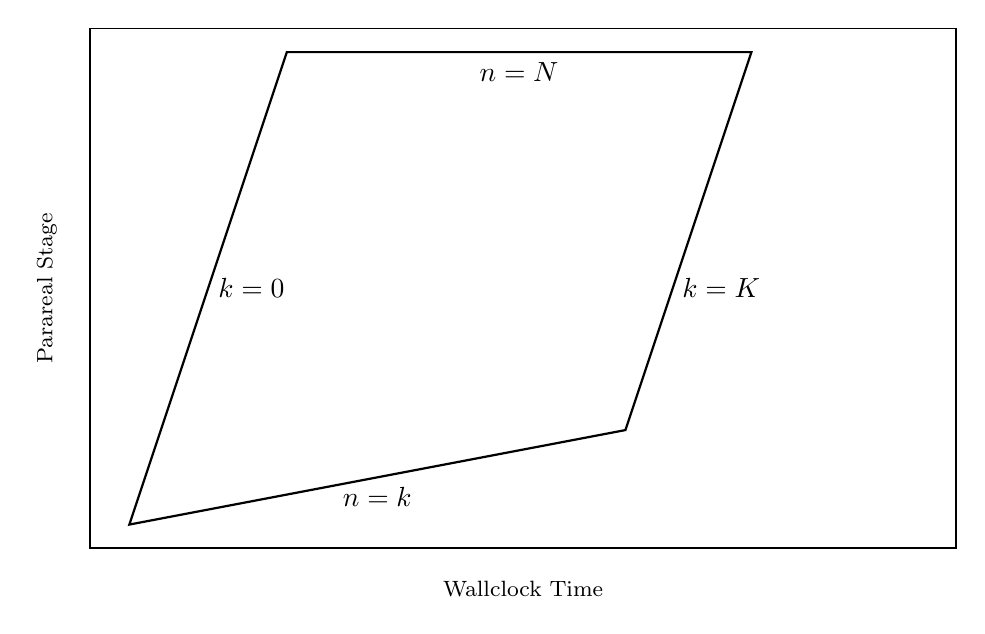
\begin{tikzpicture}
  %\def\mxscale{0.6}
  \def\myscale{0.6}
%\begin{scope}[xscale=\mxscale]
  % axis and labels
  \node[below] at (5,-0.5*\myscale-0.3) {\footnotesize Wallclock Time};
  \node[rotate=90, above] at (-0.5-0.3,5*\myscale) {\footnotesize Parareal Stage};
\begin{scope}[yscale=\myscale]
  \draw[semithick] (-0.5,-0.5) rectangle (10.5,10.5);
  % timeline diagram
  \draw[thick] (0,0)
    -- node[right] {$k=0$} (2,10)
    -- node[below] {$n=N$} (7.9,10)
    -- (6.3,2)
    -- node[below] {$n=k$} cycle;
  \node[right] at (6.9,5) {$k=K$};
  %\draw[gray,thick,dashed] (6.3,2) -- (9.45,3);
  %\draw[gray,thick,dashed] (7.9,10) -- (9.45,10);
\end{scope}
%\end{scope}
\end{tikzpicture}

  \caption[Schematic parareal timeline]{%
    Schematic parareal timeline.
    Time passed and refinement $k$ both increase to the right,
    the parareal stage $n$ increases to the top.
    The $k=K$ boundary will not be visible if $K\geq N$.
  }
  \label{fig:timeline:generic}
\end{figure}

\pagebreak

\begin{example}[Linear ODE]
\label{example:parareal}
  Let $\phi := \frac{1+\sqrt{5}}{2}$ denote the golden ratio and
  let $\kappa := \frac{2}{\pi} \log \phi$.
  Consider the \ac{IVP}
  \begin{equation}
    \label{eq:pr:linear}
    \left\{
    \begin{aligned}
      \dot u &= \begin{bmatrix}
        \kappa & -1 \\
        1 & \kappa
      \end{bmatrix} u \\
      u(0) &= \begin{bmatrix}
        -1 \\ -\kappa
      \end{bmatrix}
    \end{aligned}
    \right.
  \end{equation}
  for $t\in[0,2\pi]$.
  Let $N := 5$, $\tau := 2\pi/N$, and $t_n := n\tau$ for $n\in\Set{0,\ldots,N}$.
  Further, let $F$ and $G$ be implicit Euler schemes using step sizes $\tau/100$ and $\tau$, respectively.
  If the fine solver internally uses a finer mesh,
  by \autoref{thm:pr:conv},
  the global solution $x$ may be retrieved at that fine resolution $\tau/100$.

  \begin{figure}[tb]
    \includegraphics[width=\textwidth]{figures/fig_parareal_example.pdf}
    \caption[Parareal method applied to a linear ODE]{%
      First couple of refinements $k$ of the
      parareal method applied to the linear problem \eqref{eq:pr:linear}.
      The stages $n$ are decoded by color,
      with dots denoting $U^k_n$ and lines denoting $F(\optional{}, t_{n-1}, U^k_{n-1})$.
      The dashed gray curve represents the exact solution.
    }
    \label{fig:pr:linear}
  \end{figure}

  \autoref{fig:pr:linear} shows the first couple of iterations of the parareal method applied the problem above.
  For a fixed refinement $k$,
  the values $U^k_n \approx u(t_n)$ (represented by dots) are computed in sequence,
  \cf the horizontal traces in \autoref{fig:pr:DAG}.
  After that, the fine solutions $F(U_n^k)$ (represented by lines) can then be computed in parallel.
  The parareal method only ensures convergence of $U_n^k$.
  Therefore, before convergence is reached,
  the high-resolution trajectories are discontinues at $t_n$.
  Furthermore, note that the overall accuracy of the parareal solution is limited by the accuracy of $F$,
  which explains the remaining gap between the colored and the gray line.
\end{example}

\section{Parareal as a Multiple Shooting Method}
\label{sec:pr:newton}

The following construction is based on \citeauthor{Gander2007}~\cite{Gander2007}.
Consider again the autonomous \ac{IVP}
\begin{equation}
  \tag{\ref*{eq:IVP}}
  \left\{
  \begin{aligned}
    \dot u &= f(u) \\
    u(t_0) &= u_0
  \end{aligned}
  \right.
\end{equation}
Note that the solution $u : [t_0,t_f] \to V $ depends on the initial value $U_0$.
For a discretization $t_0 < t_1 < \ldots < t_N = t_f$
define the local problems
\begin{equation}
  \left\{
  \begin{aligned}
    \dot u_n &= f(u_n) \\
    u_n(t_n) &= U_n
  \end{aligned}
  \right.
\end{equation}
for $n \in \Set{0,\ldots,N-1}$
and determine suitable initial values $U_n$.
Watch the slight abuse of notation in $u_0$
for the initial value $u_0 \in V$
and the solution $u_0 : [t_0,t_1] \to V$ to the first local problem.
The local solutions $u_n : [t_n,t_{n+1}] \to V$ represent a global solution to the \ac{IVP}~\eqref{eq:IVP} if
\begin{equation}
  \mathcal F(U_0, \ldots, U_{N-1}) :=
  \left(
  \begin{aligned}
    U_0 &- u_0 \\
    U_1 &- u_0(t_1, U_0) \\
    &\vdotswithin{-} \\
    U_{N-1} &- u_{N-2}(t_{N-1}, U_{N-2})
  \end{aligned}
  \right)
  \overset{!}{=} 0.
\end{equation}
Let $U := (U_0, \ldots, U_{N-1})$ and $\Jac(U)$ denote the Jacobian of $\mathcal F$ at $U$.
Then, Newton's method reads
\begin{equation}
  U^{k+1} = U^k - \mathop{\Jac(U^k)^{-1}} \mathcal F(U^k)
\end{equation}
or, equivalently, avoiding the inversion of the Jacobian,
\begin{equation}
  \begin{bmatrix}
    I \\
    -\pdiff{U_0}{u_0}(t_1, U_0) & I \\
    & \ddots & \ddots \\
    && -\pdiff{U_{N-2}}{u_{N-2}}(t_{N-1}, U_{N-2}) & I
  \end{bmatrix}
  (U^{k+1} - U^k) = -\mathcal F(U^k)
  .
\end{equation}
Writing the above in separate equations yields
\begin{equation}
  \left\{
  \begin{aligned}
    U^{k+1}_0 &= u_0 \\
    U^{k+1}_n &= u_n(t_{n+1}, U^k_n) + \pdiff{U^k_n}{u_n}(t_{n+1}, U^k_n) (U^{k+1}_n - U^k_n).
  \end{aligned}
  \right.
\end{equation}
Lastly, choosing a fine propagator $F(U^k_n) := F(t_{n+1}; t_n, U^k_n) \approx u_n(t_{n+1}, U^k_n)$,
a coarse propagator $G$ according to
\begin{equation}
  \label{eq:pr:G}
  G(U^{k+1}_n) - G(U^k_n)
  \approx
  \pdiff{U^k_n}{u_n}(t_{n+1}, U^k_n) (U^{k+1}_n - U^k_n)
\end{equation}
as well as initial values $ U^0_{n+1} = G(U^0_n) $,
reveals the parareal method of \citeauthor{Baffico2002}~\cite{Baffico2002},
\begin{equation}
  \tag{\ref*{eq:pr:method} revisited}
  \left\{
  \begin{aligned}
    U_0^* &= u_0 \\
    U^0_{n+1} &= G(U^0_n) \\
    U^{k+1}_{n+1} &= F(U^k_n) + G(U^{k+1}_n) - G(U^k_n)
    .
  \end{aligned}
  \right.
\end{equation}
A Taylor expansion of $G(U^{k+1}_n) \approx u_n(t_{n+1}, U^{k+1}_n)$ around $G(U^k_n)$ justifies Equation~\eqref{eq:pr:G}.

\section{Application to \texorpdfstring{\act{LRSIF}s}{LRSIFs}}
\label{sec:pr:DRE}

Let the \acp{LRSIF}
\begin{equation}
\begin{aligned}
  G(U^{k+1}_n) &= \mathop{L_{G,k+1}} \mathop{D_{G,k+1}} \mathop{L_{G,k+1}^\T} \\
  F(U^k_n)     &= \mathop{L_{F,k}}   \mathop{D_{F,k}}   \mathop{L_{F,k}^\T} \\
  G(U^k_n)     &= \mathop{L_{G,k}}   \mathop{D_{G,k}}   \mathop{L_{G,k}^\T}
\end{aligned}
\end{equation}
be given.
Using the low-rank update formulas described in \autoref{sec:lowrank},
the parareal update \eqref{eq:pr:method} reads
\begin{equation}
  \hat L \hat D \hat L^\T :=
  \begin{bmatrix}
    L_{G,k+1} &
    L_{F,k} &
    L_{G,k}
  \end{bmatrix}
  \begin{bmatrix}
    D_{G,k+1} \\
    & D_{F,k} \\
    && -D_{G,k}
  \end{bmatrix}
  \begin{bmatrix}
    L_{G,k+1}^\T \\
    L_{F,k}^\T \\
    L_{G,k}^\T
  \end{bmatrix}
  .
\end{equation}
Note the downdate in the last block component.
The actual low-rank representation of~$U^{k+1}_{n+1}$ is set to a column compression of~$\hat L \hat D \hat L^\T$
using \autoref{alg:lowrank:compression}.

%\section{Alternative Parallel-in-Time Solvers}
